\chapter{RFX-Hunch: a closed example based on electron temperature}
\label{section:RFXhunch}

With the aim at selecting an informative example of plasma computation that the machine learning could be devoted to, we chose to look at the temperature profiles that are coming from the Soft X-Ray diagnostics at RFX. The particular choice had been mainly motivated by the fact that it provides an example that can be a good representative factor of the plasma global configuration, being at the same time not too complex to be handled by simple networks. The electron temperature profile represents indeed a very important clue for looking at the plasma state that is very often accessed by physicists during analysis: it can be seen as an instant property that is almost ergodic during the pulse, it is acquired with a good temporal resolution, and that can be related to the magnetic configuration for the chosen time sample.

A plasma is composed with a mixture of species characterized by their own mass and electric charge. As first approximation, the plasma may be considered as consisting of two fluids mixed together: the first composed by the electrons and the second by the ions, or to be more specific by all the other heavy species: ions, neutral atoms, and other compound molecules.

What matters for a fusion machine is actually the ions temperature because electrons are not directly involved on fusion process.
Nevertheless electrons acquire energy from the electric field, which energizes the plasma, and lose part of it through elastic or inelastic collisions; in this way the plasma can move energy from one fluid to the other. For this reason in \textit{Tokamaks} this represents a direct handle for plasma heating through \acs{ECRH} plants. In RFX we don't have such input and the electron temperature are almost directly related to the plasma current and the magnetic pressure (\textit{pinch} effect).
In addition the acquired profile represents a local information of the internal state of plasma giving a chance to see through the simple external configuration.

This holds for the Thomson scattering too, indeed: the SXR invese-transformed profile of the plasma bremsstrahlung radiation, and the intensity of the scattered light from TS, provide the same kind of measure being both of them related to electrons velocity.
However, as already discussed, the two diagnostics are not interchangeable as they present different characteristics. In particular the TS is known to provide a more accurate measure both in spatial resolution and in the accuracy of the acquired quantity; on the other hand the SXR measure even being quite noisy, easily biased by plasma-wall interaction debris of carbon and other materials, and usually presenting a set of reconstructed points that vary in position and in number, has a very fine grained resolution in the time domain.
In RFX we have the SXR3 time resolution of about $500 \mu s$

\section{What involved ( based on “SCHEMA” )} % SHAx




%% FD-NT-27
\section{Passing from simulated data to actual data  “missing points”  }

\begin{figure}
    \centering
    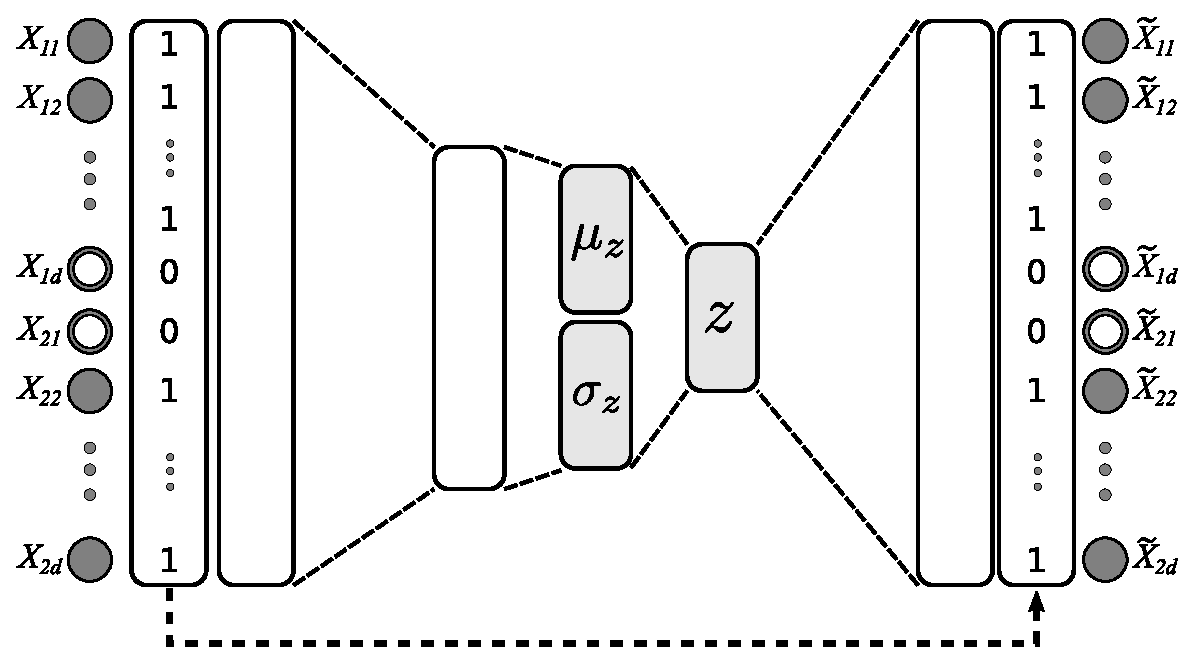
\includegraphics[height=6cm]{img/6_T_Hunch/VAE_MISSING.eps}
    \caption{VAE Missing point training NaN-Mask layer}
    \label{fig:6_vae_missing}
\end{figure}



\begin{figure}
    \centering
    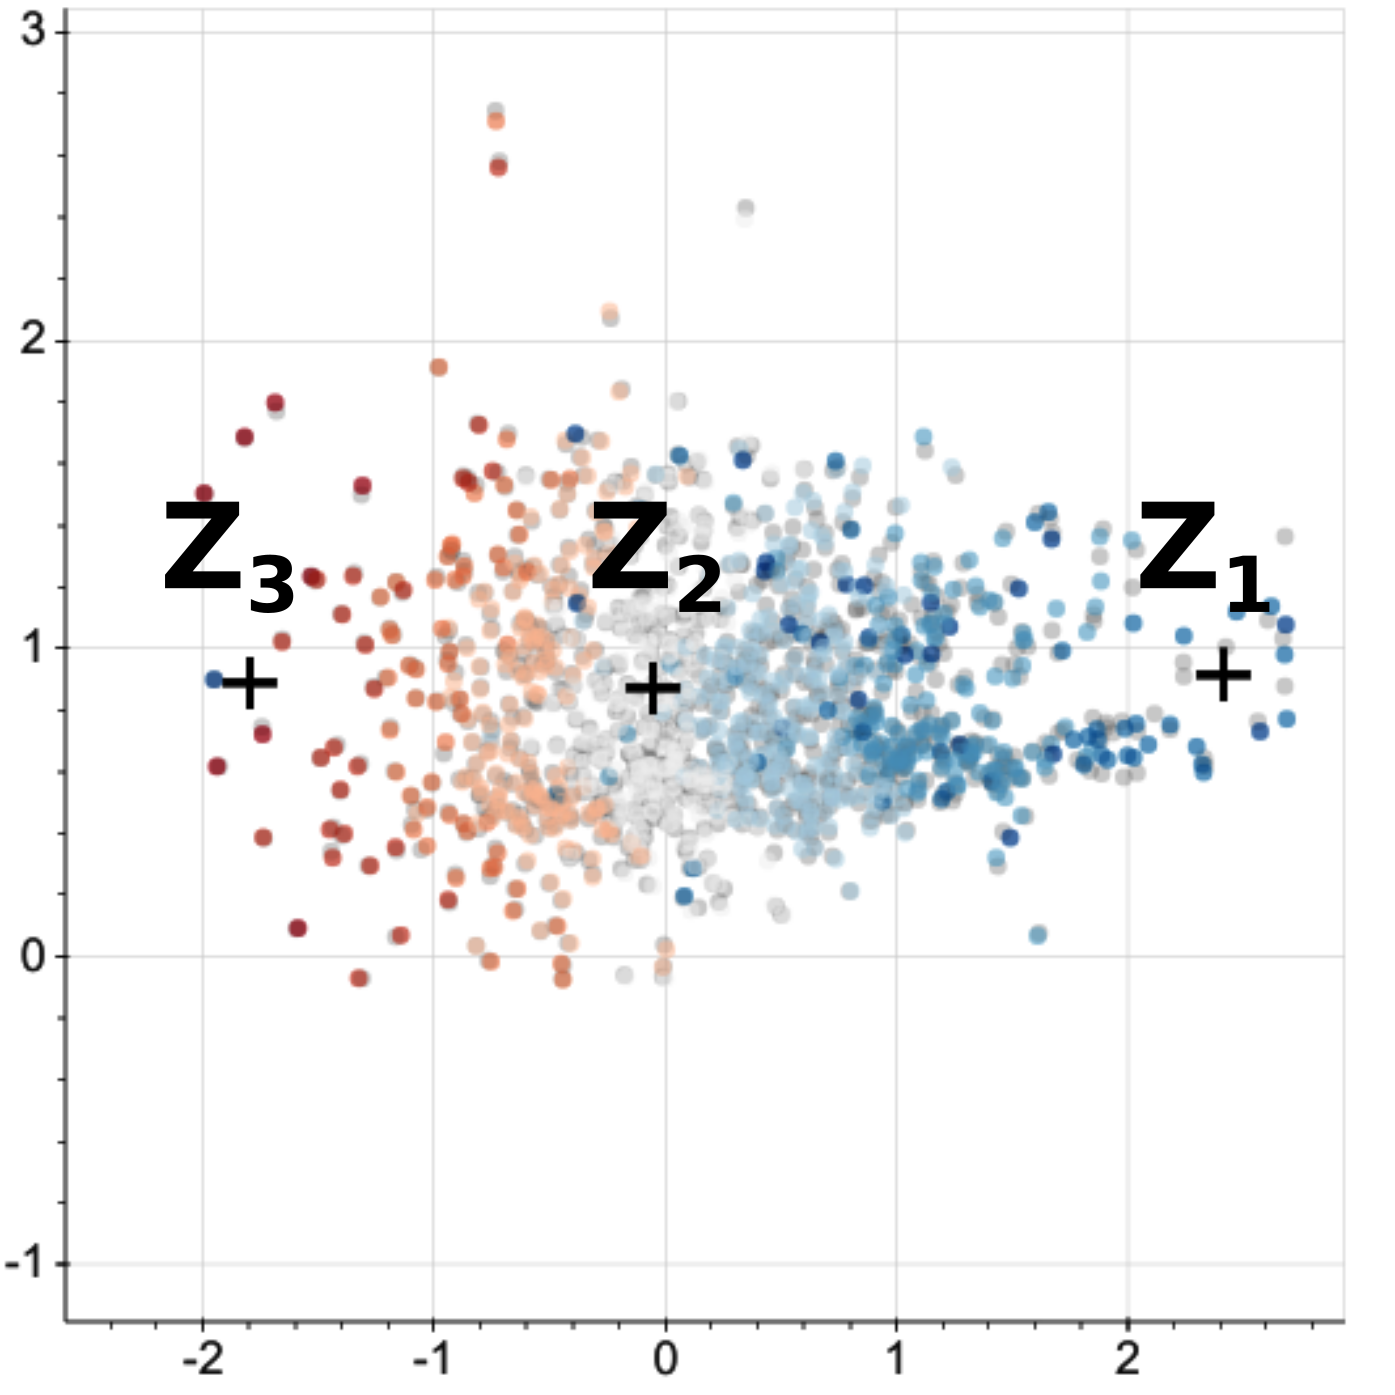
\includegraphics[height=6cm]{img/6_T_Hunch/ls_beta_tcentro_123.png}
    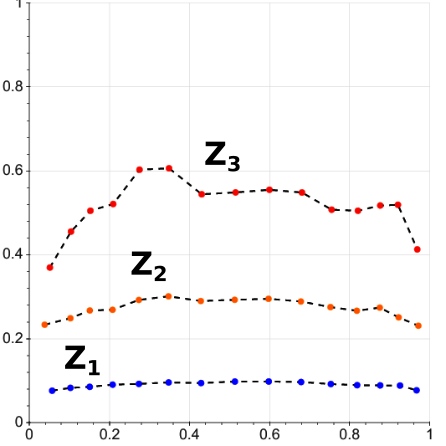
\includegraphics[height=6cm]{img/6_T_Hunch/ls_beta_tcentro_123_gen.png}
    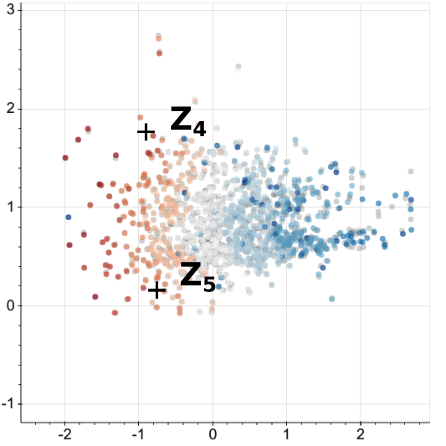
\includegraphics[height=6cm]{img/6_T_Hunch/ls_beta_tcentro_45.png}
    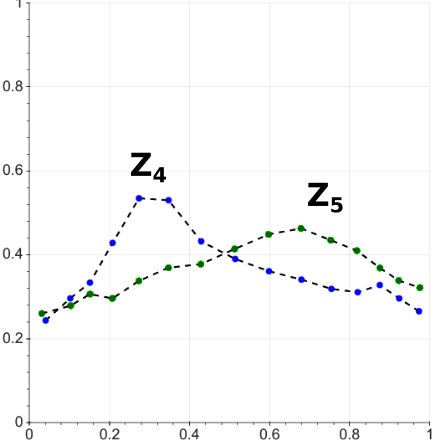
\includegraphics[height=6cm]{img/6_T_Hunch/ls_beta_tcentro_45_gen.png}
    \caption{VAE tcentro}
    \label{fig:my_label}
\end{figure}


\begin{figure}
    \centering
    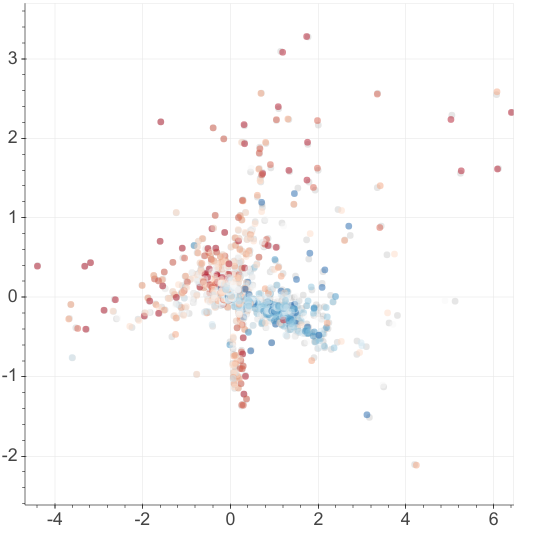
\includegraphics[height=6cm]{img/6_T_Hunch/ls_beta_clip_tcentro.png}
%    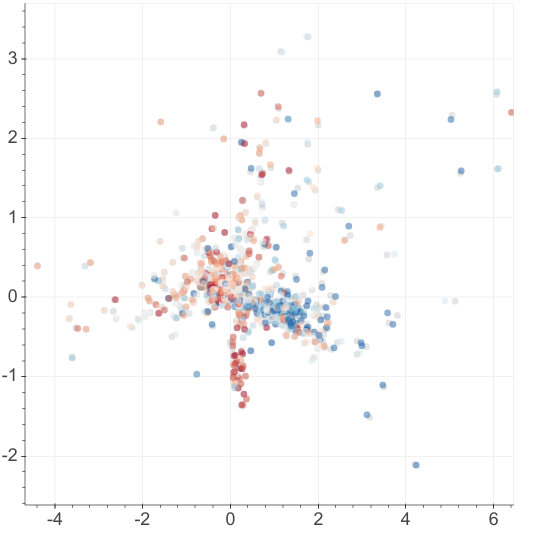
\includegraphics[height=6cm]{img/6_T_Hunch/ls_beta_clip_tbordo.png}
    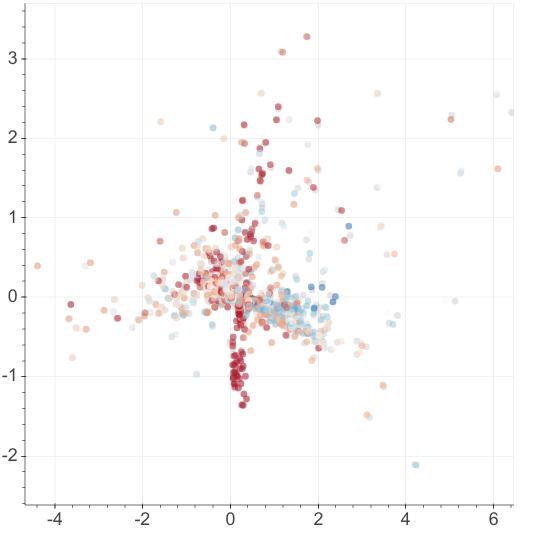
\includegraphics[height=6cm]{img/6_T_Hunch/ls_beta_clip_Ip.png}
    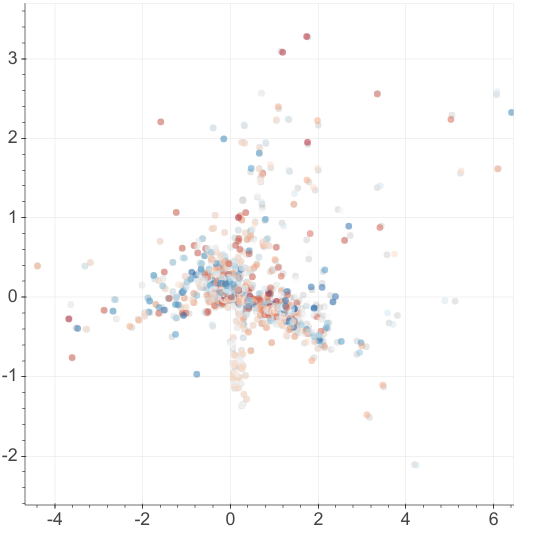
\includegraphics[height=6cm]{img/6_T_Hunch/ls_beta_clip_F.png}
    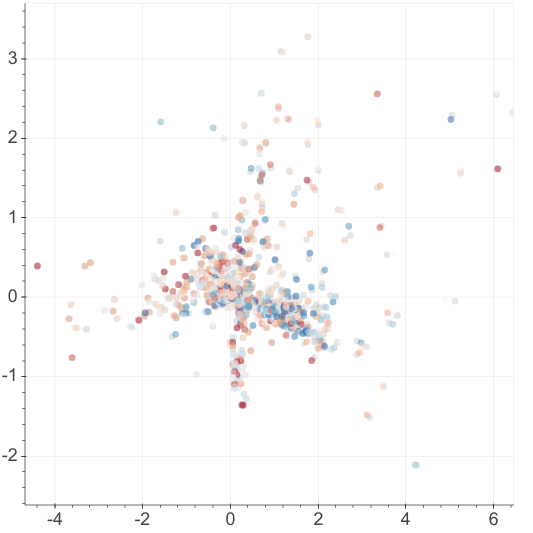
\includegraphics[height=6cm]{img/6_T_Hunch/ls_beta_clip_NS.png}
    \caption{VAE clip vs external info}
    \label{fig:my_label}
\end{figure}

\begin{figure}
    \centering
    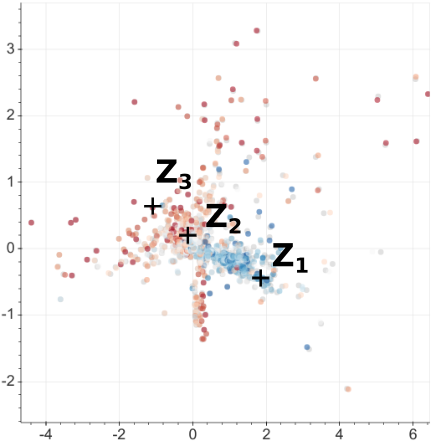
\includegraphics[height=6cm]{img/6_T_Hunch/ls_beta_clip_tcentro_123.png}
    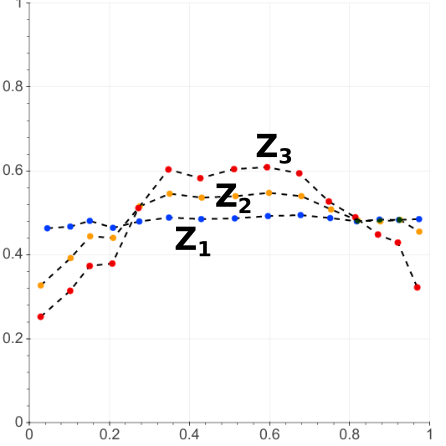
\includegraphics[height=6cm]{img/6_T_Hunch/ls_beta_clip_tcentro_123_g.png}
    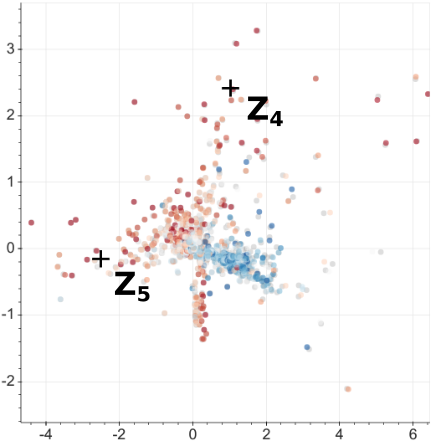
\includegraphics[height=6cm]{img/6_T_Hunch/ls_beta_clip_tcentro_45.png}
    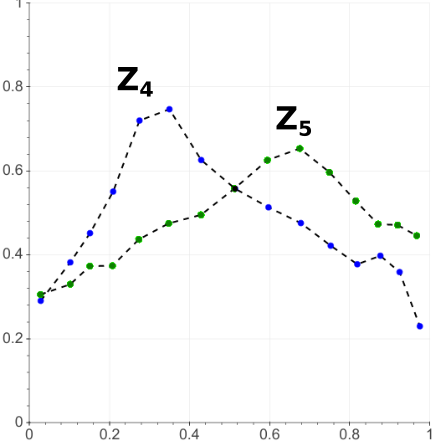
\includegraphics[height=6cm]{img/6_T_Hunch/ls_beta_clip_tcentro_45_g.png}
    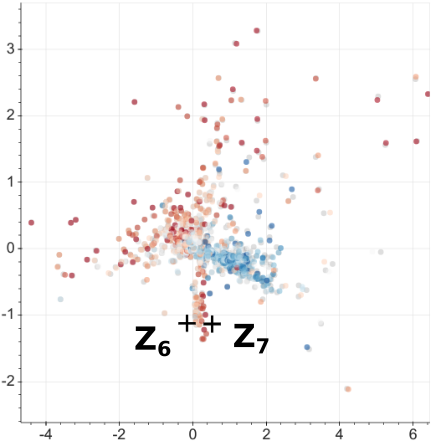
\includegraphics[height=6cm]{img/6_T_Hunch/ls_beta_clip_tcentro_67.png}
    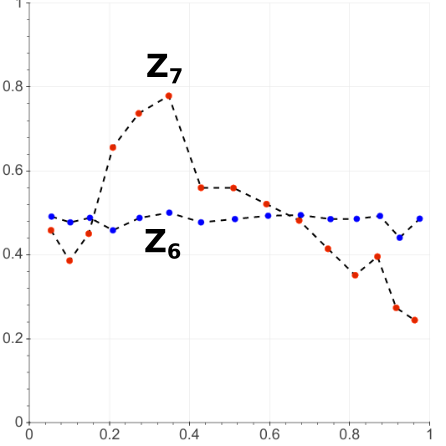
\includegraphics[height=6cm]{img/6_T_Hunch/ls_beta_clip_tcentro_67_g.png}
    \caption{VAE clip space}
    \label{fig:my_label}
\end{figure}

\section{( show using of dropout, rebalancing and beta )}






\section{parameters to SXR mapping}



\section{Adding information through models ( Zanca-Terranova )}


\begin{figure}
    \centering
    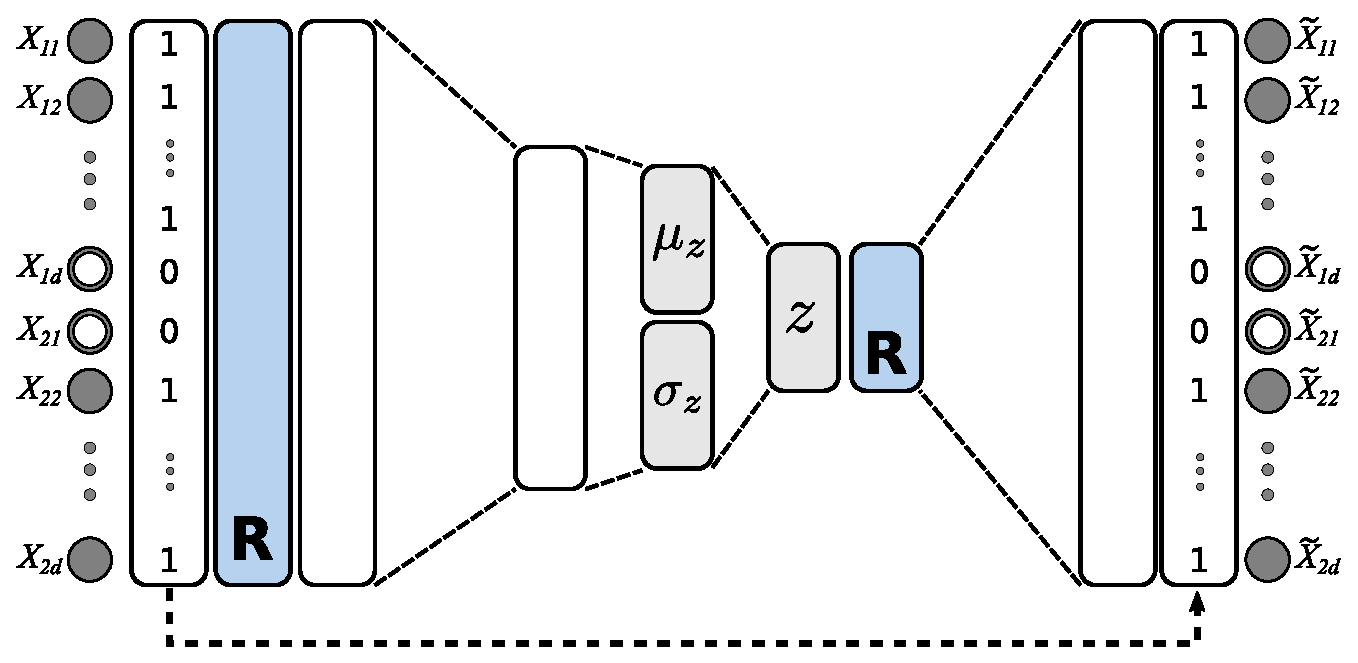
\includegraphics[height=6cm]{img/STEP12_7/VAE_RELEVANCE.eps}
    \caption{Relevance layer}
    \label{fig:my_label}
\end{figure}

\begin{figure}
    \centering
    \subfigure{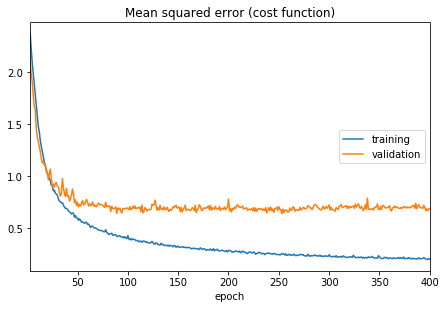
\includegraphics[height=3.3cm]{img/STEP12_7/STEP12_7_pBr2SXR_rm-rs_absarg_training_mse.png} \label{step_12_7_training}}
    \subfigure{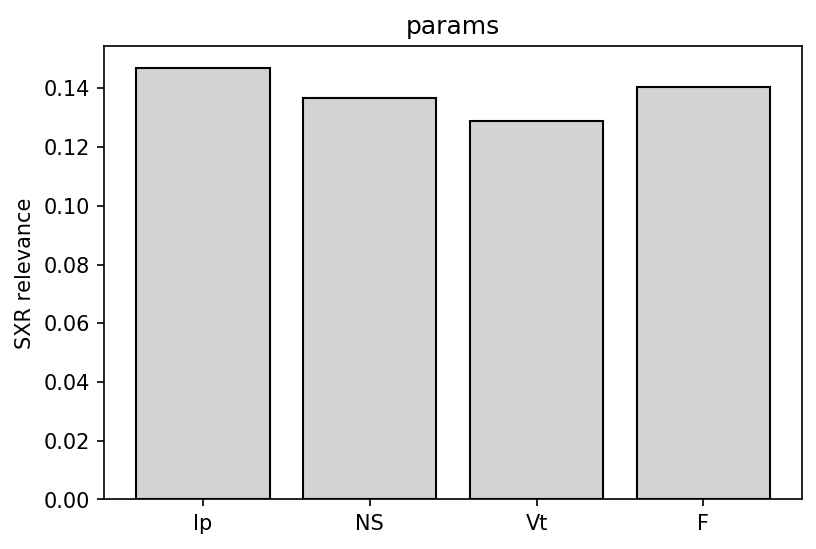
\includegraphics[height=3.3cm]{img/STEP12_7/STEP12_7_params.png} \label{step_12_7_p}}
    \subfigure{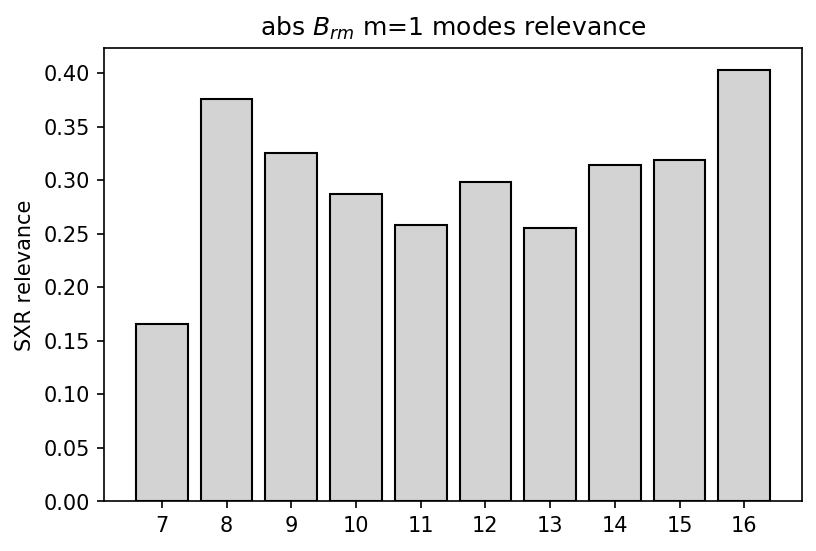
\includegraphics[height=3.3cm]{img/STEP12_7/STEP12_7_abs_Br_rm.png} \label{step_12_7_abs_Brm}}
    \subfigure{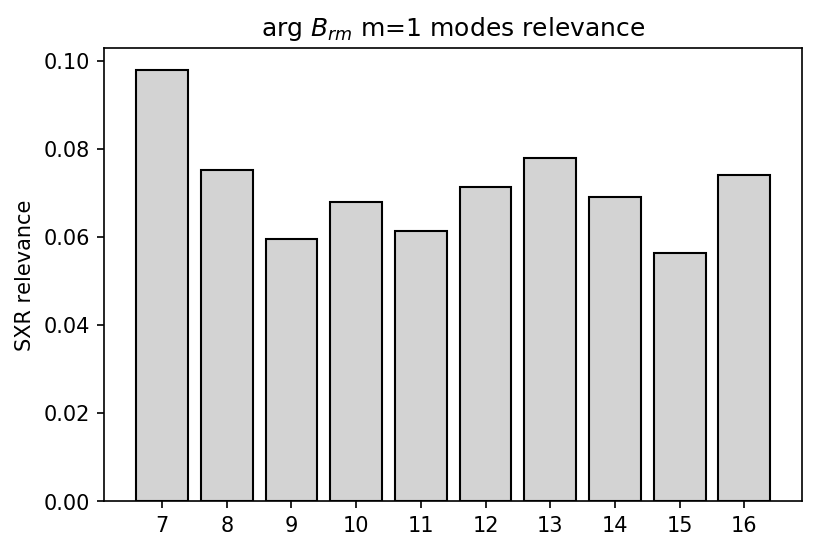
\includegraphics[height=3.3cm]{img/STEP12_7/STEP12_7_arg_Br_rm.png} \label{step_12_7_arg_Brm}}
    \subfigure{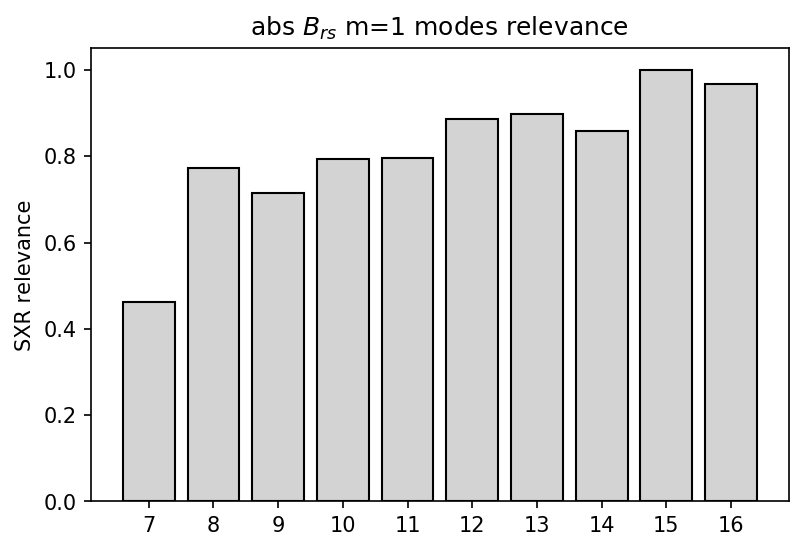
\includegraphics[height=3.3cm]{img/STEP12_7/STEP12_7_abs_Br_rs.png} \label{step_12_7_abs_Brs}}
    \subfigure{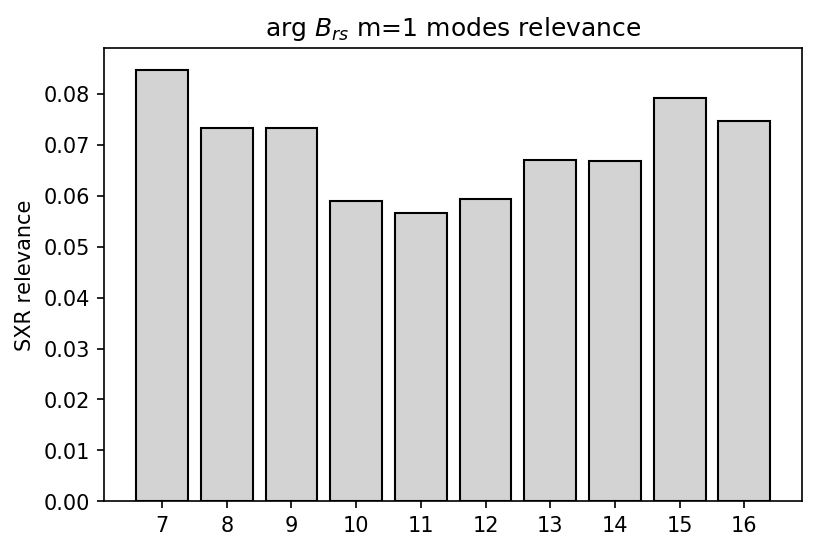
\includegraphics[height=3.3cm]{img/STEP12_7/STEP12_7_arg_Br_rs.png} \label{step_12_7_arg_Brs}}
    \caption{ Training 500 epochs - STEP 12.7 mse, slightly overfitted but validation not diverging }
    \label{fig:step_12_7}
\end{figure}

\begin{figure}
    \centering
    \subfigure{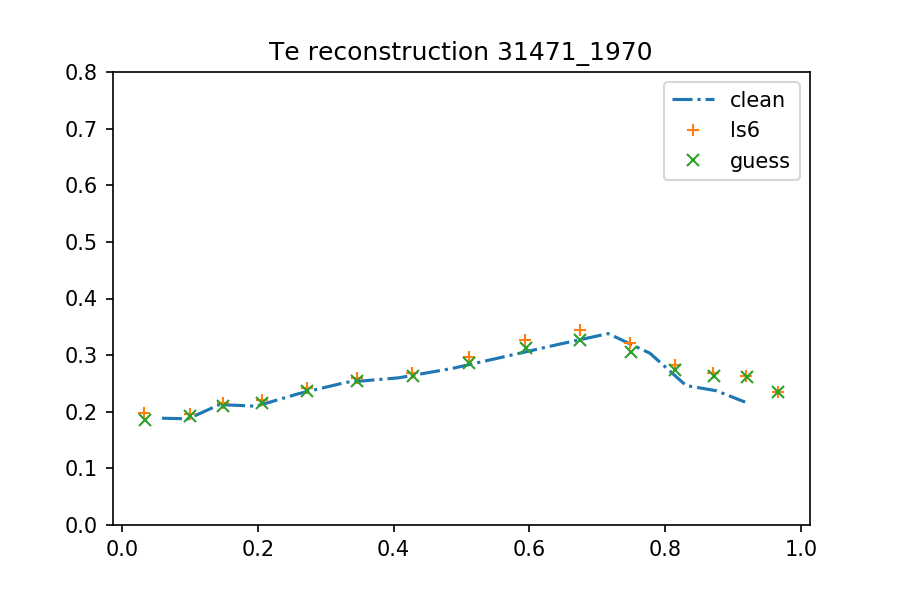
\includegraphics[height=4.8cm]{img/STEP12_7/Te_rec_215.png} }
%   \subfigure{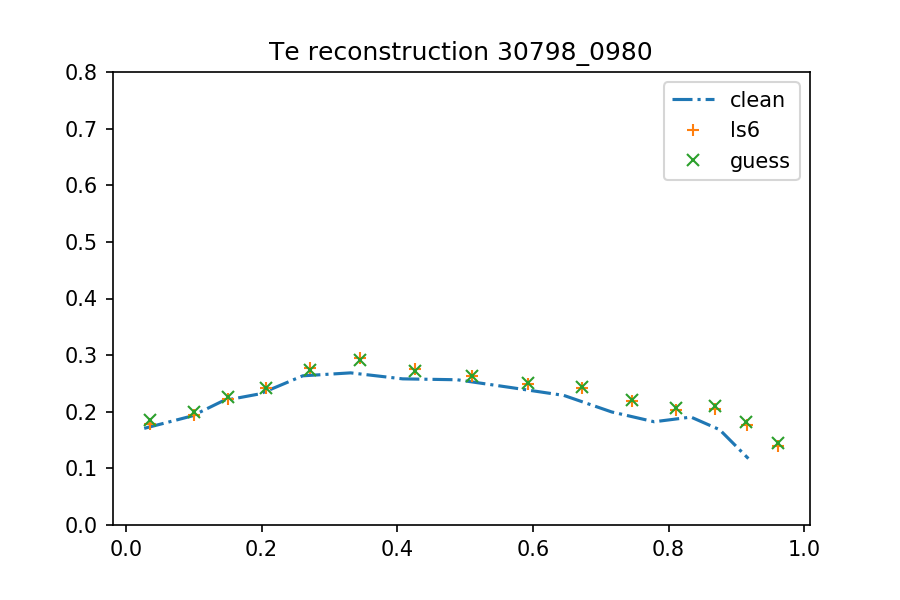
\includegraphics[height=4.8cm]{img/STEP12_7/Te_rec_219.png} }
    \subfigure{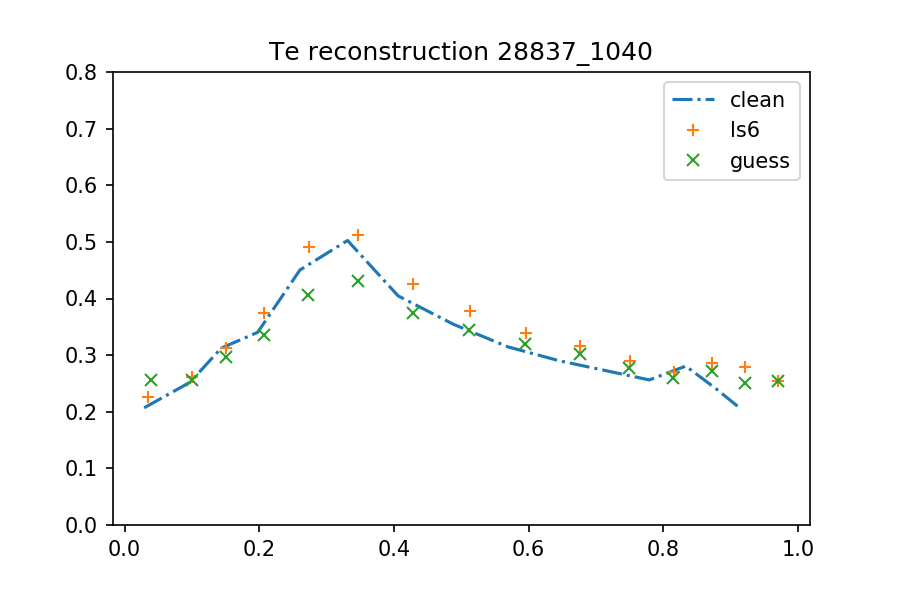
\includegraphics[height=4.8cm]{img/STEP12_7/Te_rec_229.png} }
    \subfigure{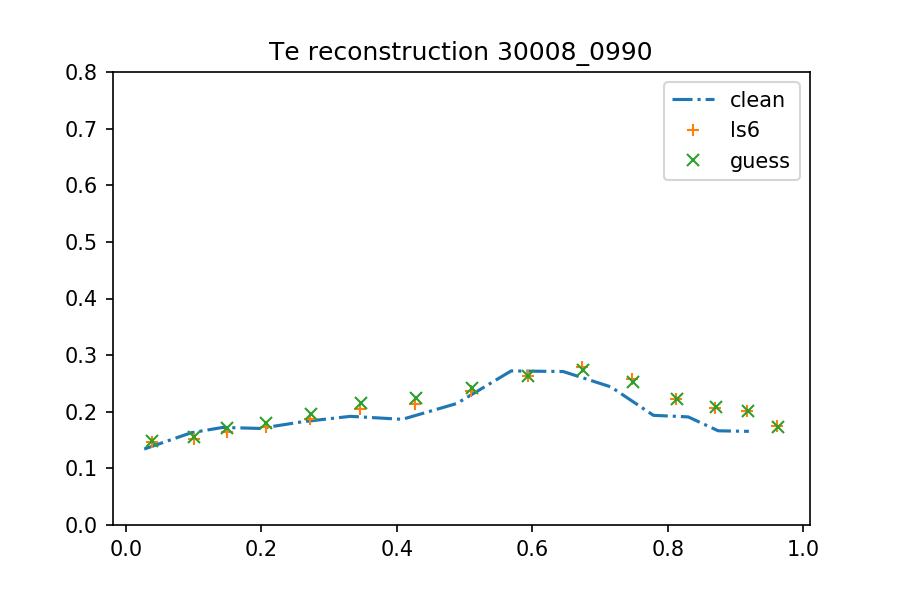
\includegraphics[height=4.8cm]{img/STEP12_7/Te_rec_232.png} }
%   \subfigure{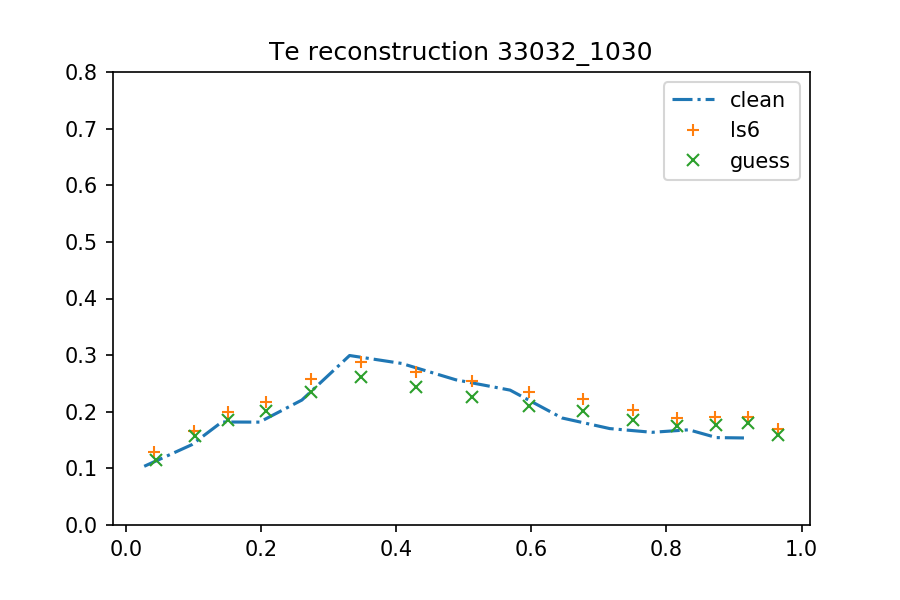
\includegraphics[height=4.8cm]{img/STEP12_7/Te_rec_243.png} }
    \subfigure{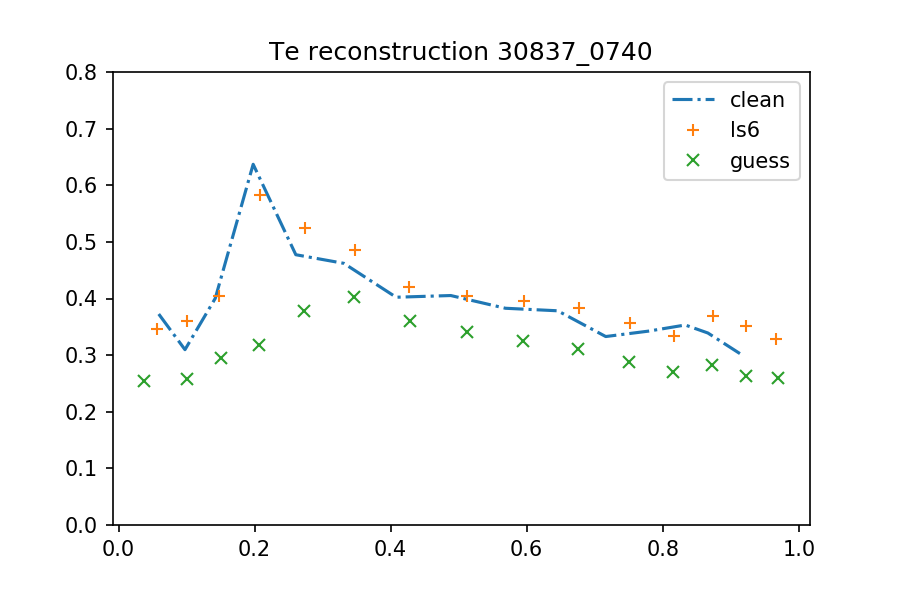
\includegraphics[height=4.8cm]{img/STEP12_7/Te_rec_213.png} }
    \caption{ Training 500 epochs - STEP 12.7 mse, slightly overfitted but validation not diverging }
    \label{fig:step_12_7_rec}
\end{figure}

